\documentclass[
aspectratio=169,
16pt,
xcolor={dvipsnames} % https://tex.stackexchange.com/a/74807
]{beamer}

\usepackage{amsfonts}
\usepackage{amsmath}
\usepackage{wrapfig}
\usepackage{physics} 
\usepackage{mathtools} 
\usepackage{qrcode}
\usepackage[russian]{babel} %Comment this line and delete all russian text for ENGLISH
\usepackage{graphicx} % Allows including images
\usepackage{tikz}

% bibliography
\usepackage[
	backend=biber,
	style=science,  % usually the most compact
	sorting=none,
]{biblatex}
\addbibresource{references.bib}

% change footnote size font 
% https://tex.stackexchange.com/a/146021
\setbeamerfont{footnote}{size=\tiny}


% fontsize at the end
\AtBeginBibliography{\small}

% https://en.wikibooks.org/wiki/LaTeX/Colors
\newcommand{\blue}[1]{\textcolor{NavyBlue}{#1}}
\newcommand{\red}[1]{\textcolor{BrickRed}{#1}}
\newcommand{\green}[1]{\textcolor{green!50!black}{#1}}
\newcommand{\white}[1]{\textcolor{white}{#1}}

% ------------
% themes
% ------------
%\usetheme{default}
%\usetheme{AnnArbor}
%\usetheme{Antibes}
%\usetheme{Bergen}
%\usetheme{Berkeley}
%\usetheme{Berlin}
%\usetheme{Boadilla} % !
%\usetheme{CambridgeUS} % !
%\usetheme{Copenhagen}
%\usetheme{Darmstadt}
%\usetheme{Dresden}
%\usetheme{Frankfurt}
\usetheme[left]{Goettingen} % !!
%\usetheme{Hannover} % !
%\usetheme{Ilmenau}
%\usetheme{JuanLesPins}
%\usetheme{Luebeck}
%\usetheme{Madrid} % !
%\usetheme{Malmoe} % !
%\usetheme{Marburg} % !
%\usetheme{Montpellier}
%\usetheme{PaloAlto}
%\usetheme{Pittsburgh} 
%\usetheme{Rochester}
%\usetheme{Singapore} % !!
%\usetheme{Szeged}
%\usetheme{Warsaw}

% ------------
% colors
% ------------
%\usecolortheme{albatross}
%\usecolortheme{beaver}
%\usecolortheme{beetle}
%\usecolortheme{crane}
%\usecolortheme{dolphin}
%\usecolortheme{dove} % !
%\usecolortheme{fly}
%\usecolortheme{lily}
%\usecolortheme{orchid}
%\usecolortheme{rose}
\usecolortheme{seagull} % !
%\usecolortheme{seahorse}
%\usecolortheme{whale}
%\usecolortheme{wolverine}
\AtEveryCitekey{
  \clearfield{issn} %don't show this in citations
  \clearfield{note}
}


% ------------
% extra theme settings
% ------------

% colors of navigation bar
% https://tex.stackexchange.com/questions/246201/color-of-the-navigation-bar-in-beamer-theme-goettingen
\makeatletter
\setbeamertemplate{sidebar canvas \beamer@sidebarside}[vertical shading][top=BurntOrange!25,bottom=BrickRed!10]
\makeatother

% Look of the block enviroment
\setbeamercolor{block title}{bg=BurntOrange!25}
\setbeamercolor{block body}{bg=BrickRed!5}

% change this if you make titles bold by default
%\setbeamertemplate{frametitle}{\vspace{0.3cm}\textcolor{BrickRed}{\textbf{\insertframetitle}}}

% remove the navigation symbols
\setbeamertemplate{navigation symbols}{} 

% adds slide numbers
\addtobeamertemplate{navigation symbols}{}{%
	\usebeamerfont{footline}%
	\usebeamercolor[fg]{footline}%
	\hspace{1em}%
	\insertframenumber/\inserttotalframenumber
}

\addtobeamertemplate{frametitle}{}{%
\begin{tikzpicture}[remember picture,overlay]
	\node[anchor=north east,yshift=2pt] at (current page.north east) {\includegraphics[height=0.7cm]{fig/logo}};
\end{tikzpicture}}


%\pgfdeclareimage[height=1.3cm]{uni}{fig/logo}
\logo{\pgfuseimage{uni}}



%-------------------
%	title settings
%-------------------

\title[Short title]{\textbf{Long (long  long long long long long) title}} 

\author[Ivan Toftul]{
	\textbf{Ivan Toftul}, 
	Your Colleagues, ...
} 

\institute[ITMO]{
	Faculty of Physics, ITMO University \\ 
	\medskip
	\texttt{toftul.ivan@gmail.com} 
}
\date{
	\small{\today \\ EVENT @ PLACE}
} 


\begin{document}
	
\begin{frame}
	\titlepage 
\end{frame}

\section{Introduction}

\begin{frame}[t]{Introduction}
	\begin{columns}
		\begin{column}{0.4\linewidth}
			\begin{itemize}
				\item Don't forget to cite everything, that you haven't done by youself
				\item \green{Если картинку рисовали не вы, должна быть ссылка}
				\item Пример QR-кода \qrcode[hyperlink,height=0.5in]{https://clck.ru/vzHWc}
			\end{itemize}
		\end{column}
		\begin{column}{0.6\linewidth}
			\begin{figure}
				\includegraphics[width=1.0\linewidth]{fig/harmonicscalibri0}
				{\raggedright\tiny Source:~\fullcite{Gladyshev2022-Boundstatesinthec}\par}
			\end{figure}
		\end{column}
	\end{columns}
\end{frame}

\begin{frame}[t]{Relevance of the work}
	\begin{columns}
		\begin{column}{0.2\linewidth}
			\begin{itemize}
				\item One
				\item Two
				\item Three				
			\end{itemize}
		\end{column}
		\begin{column}{0.3\linewidth}
			\begin{figure}
				
\includegraphics[width=1.0\linewidth]{fig/Vector_fig}
				\caption{Nice Utia}
				 {\raggedright\tiny Source: \fullcite{Utia}\par}
			\end{figure}
		\end{column}
		\begin{column}{0.4\linewidth}
			\begin{figure}
				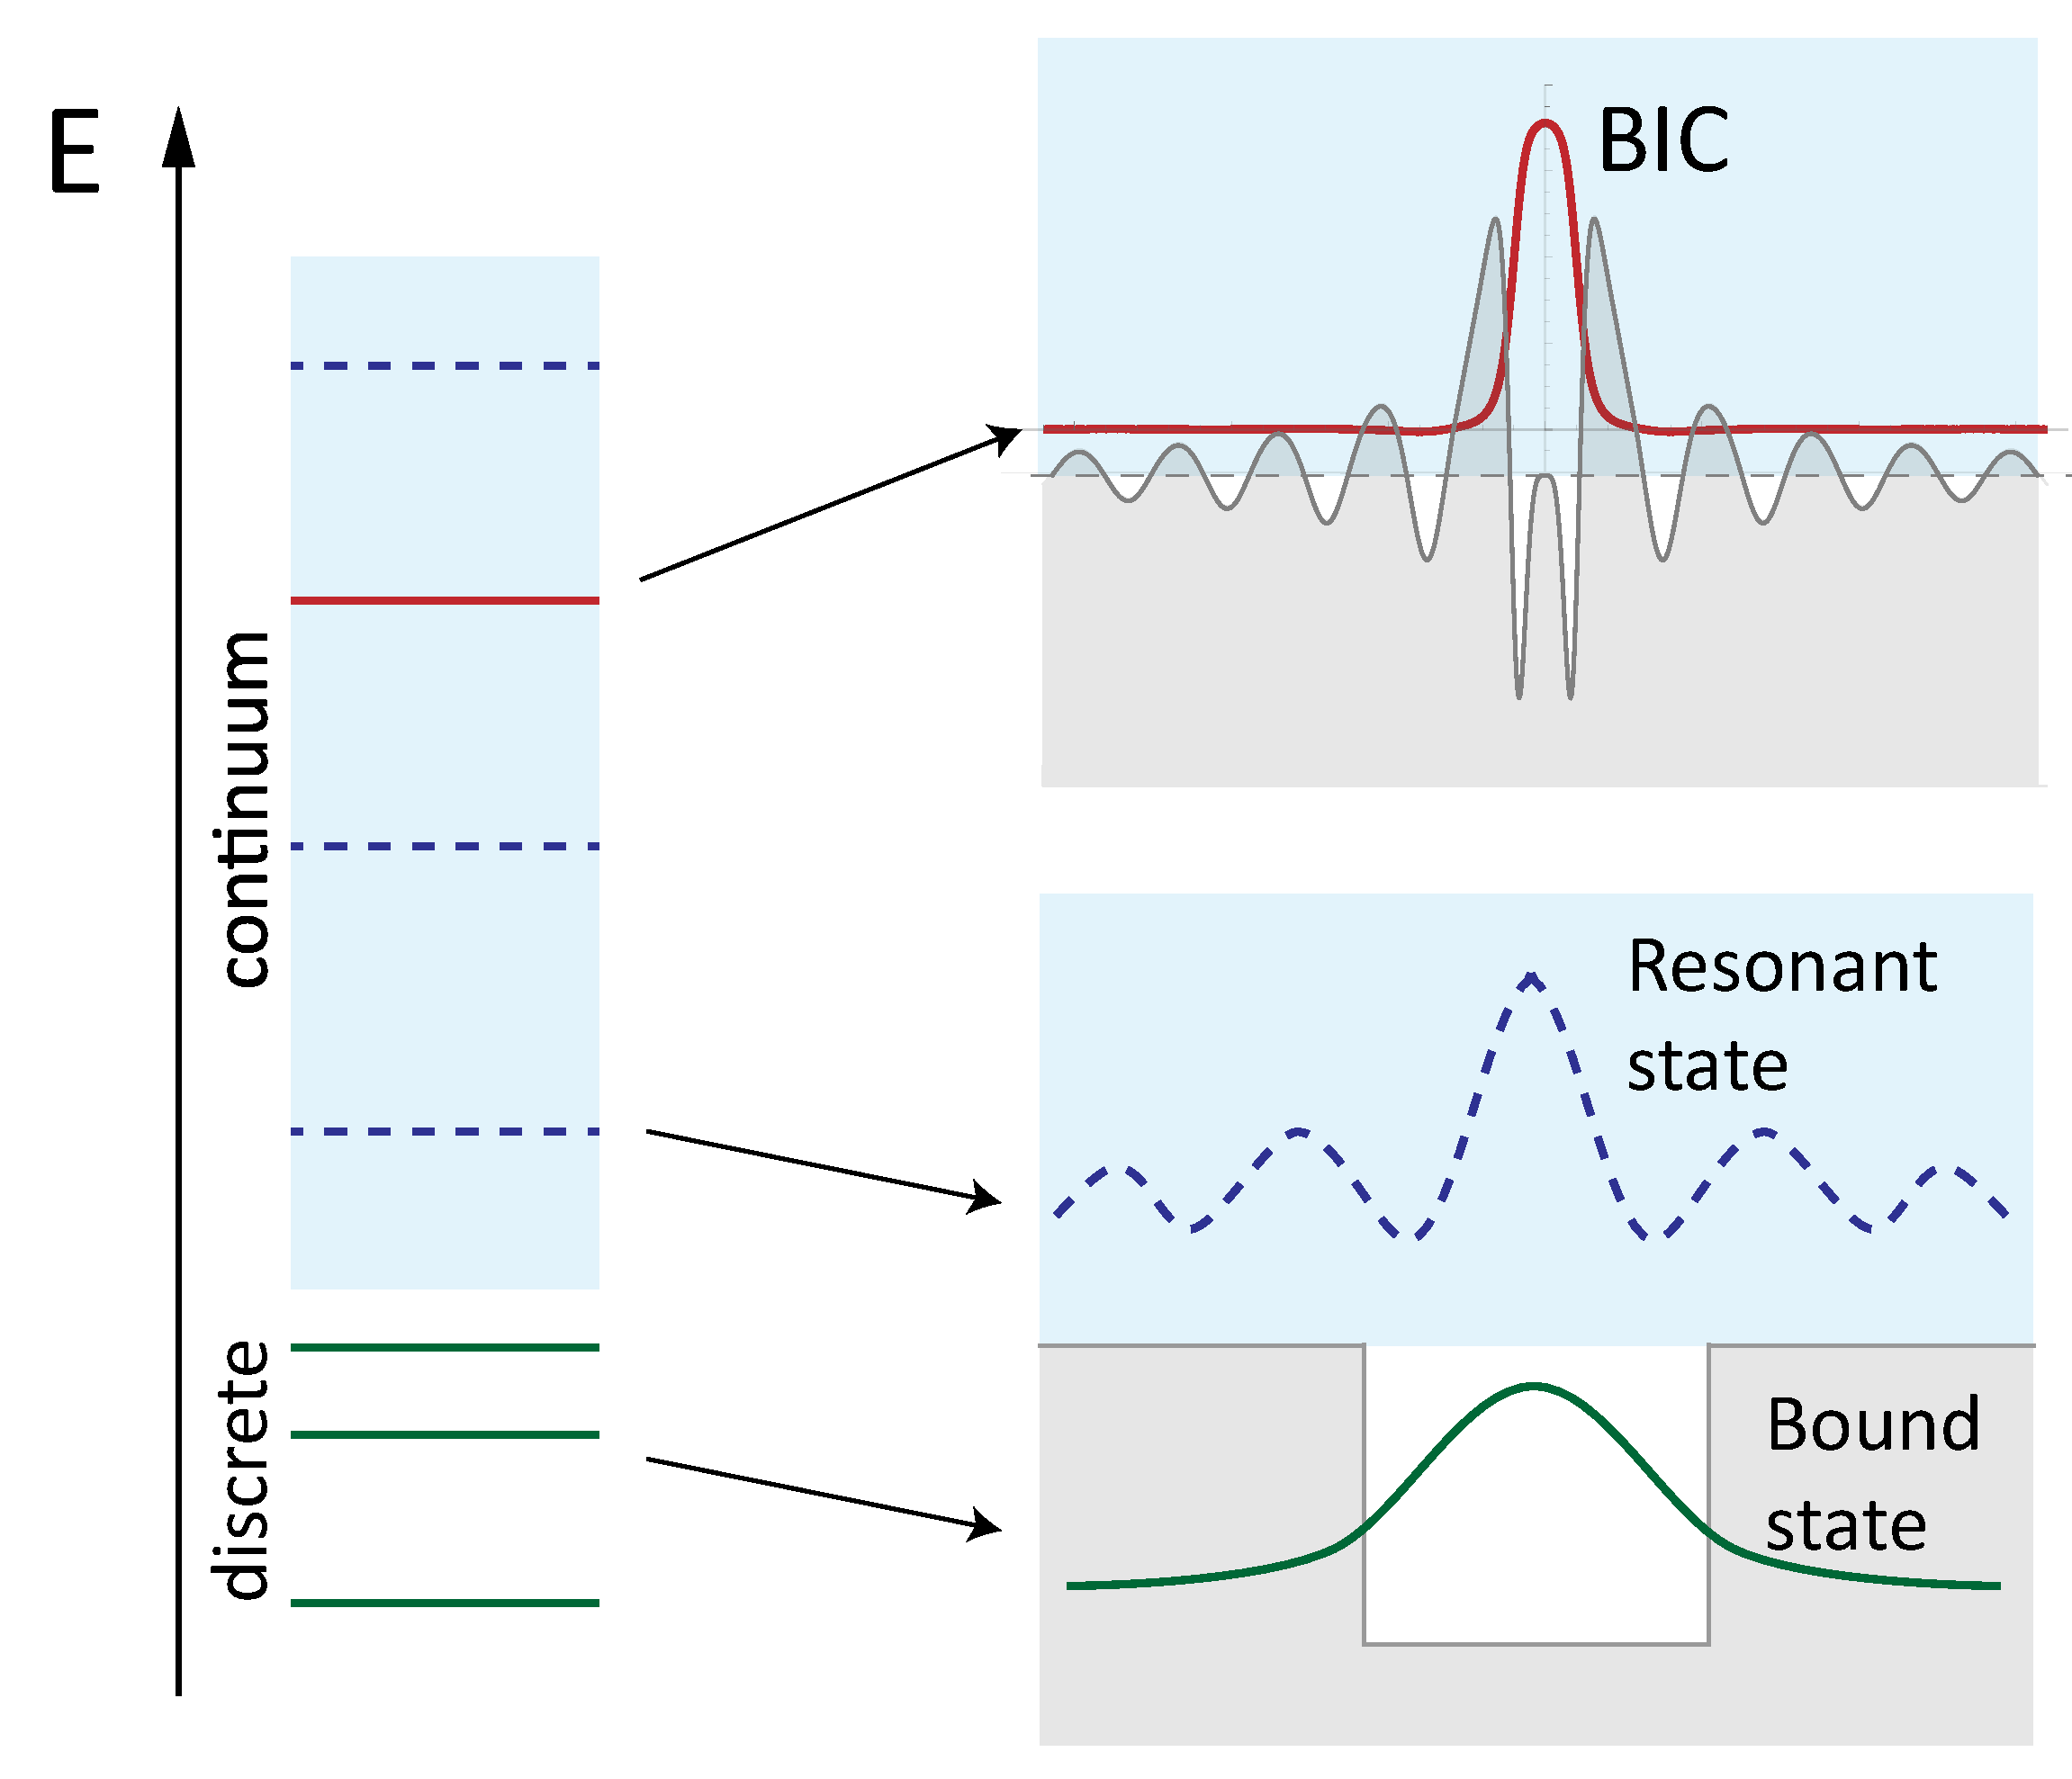
\includegraphics[width=0.9\linewidth]{fig/bicwiki0}
				\caption{BIC Illustration}
				 {\raggedright\tiny Source:\fullcite{BICwiki}\par}
			\end{figure}
		\end{column}
	\end{columns}
\end{frame}

\section{Постановка задачи}
\begin{frame}[t]{Постановка задачи}
	\begin{figure}
      
				\includegraphics[width=0.4\linewidth]{fig/scheme.png}
				\caption{Схема установки/иллюстрация основной идеи/геометрия задачи~\footfullcite{Wigner}}
	\end{figure}
	Какой-то текст, или, например, формула $\int\limits_{-\infty}^\infty  e^{-x^2} \dd x=\sqrt\pi$
\end{frame}



\section{Results}
\subsection{First}
\begin{frame}[t]{First slide with results}
	From \footfullcite{Muldoon1996Feb} we have
	\[
		\sin(x) \approx x
	\]
	\begin{block}{Example}
		For $x = 0.1$ we have 
		\[
			\sin (0.1) = 0.09983341664682815
		\]
	\end{block}
\end{frame}

\subsection{Second}
\begin{frame}[t]{Second slide with results}
	\begin{columns}
		\begin{column}{0.4\linewidth}
			\begin{itemize}
				\item One
				\item Two
				\item Three				
			\end{itemize}
		\end{column}
		\begin{column}{0.4\linewidth}
			\begin{figure}
				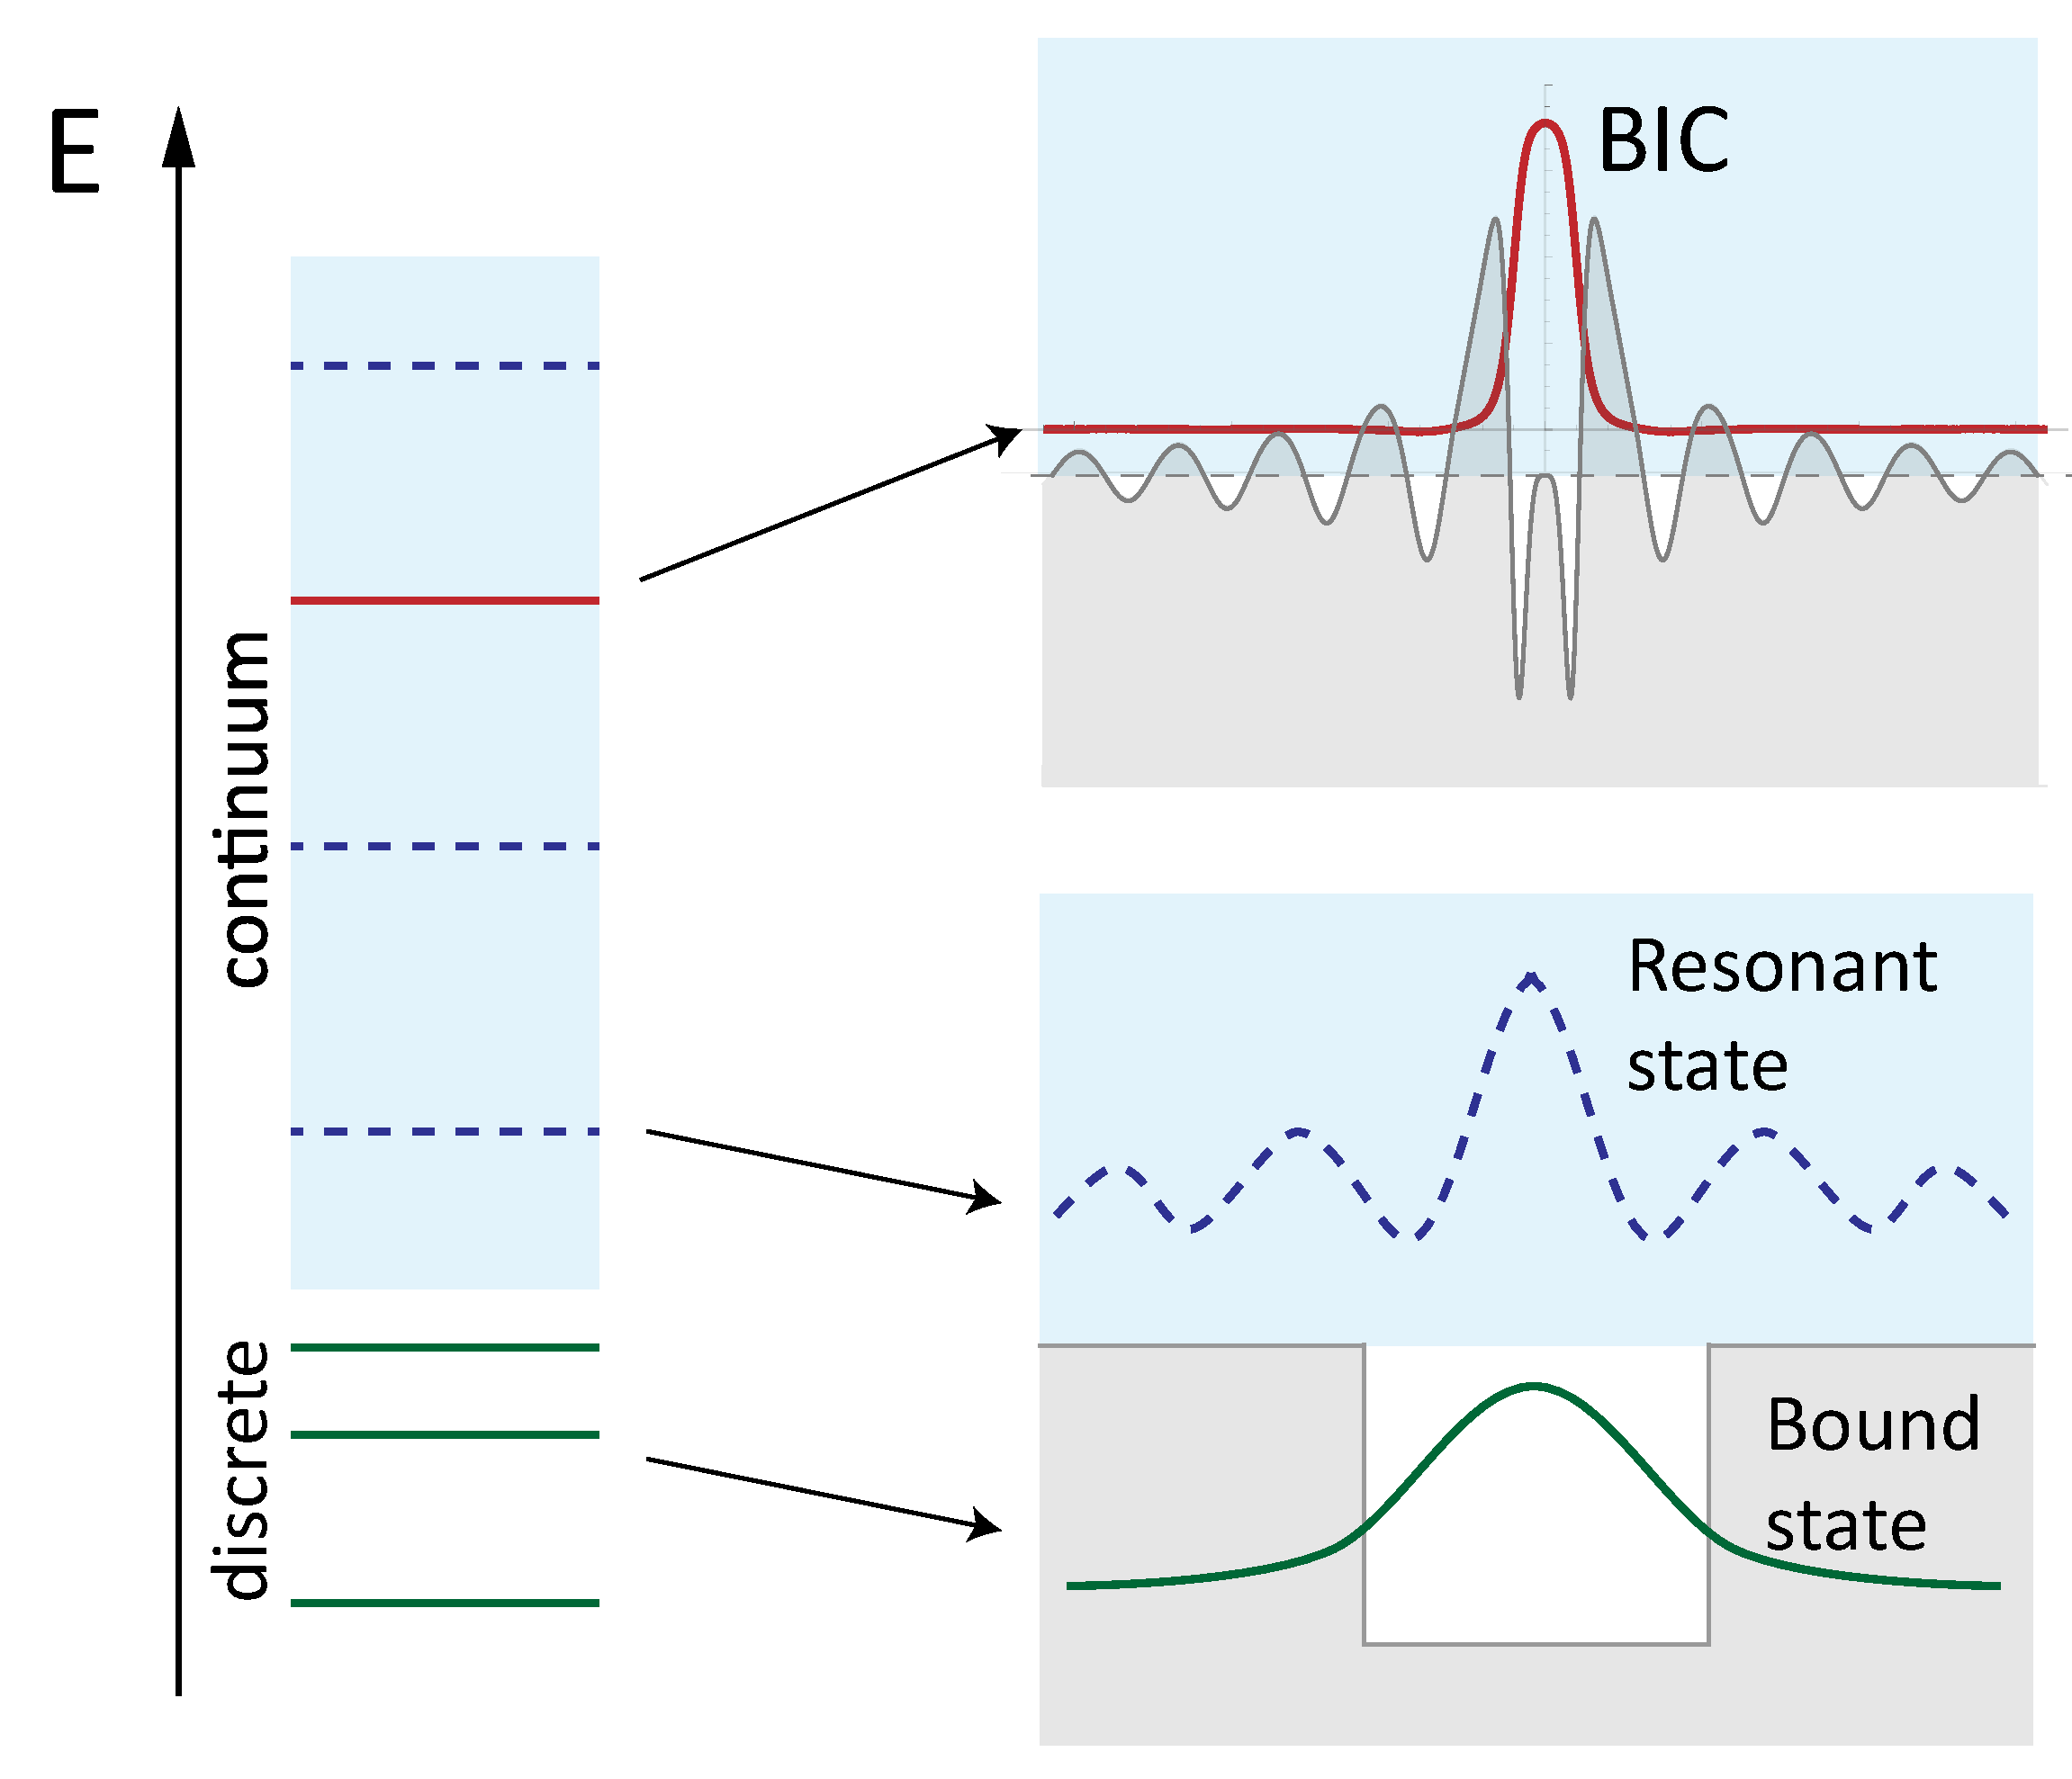
\includegraphics[width=0.9\linewidth]{fig/bicwiki0}
				\caption{BIC Illustration}
				 {\raggedright\tiny Source:\fullcite{BICwiki}\par}
			\end{figure}
		\end{column}
	\end{columns}
\end{frame}

\section{Conclusion}
\begin{frame}[t]{Conclusions}
	\begin{enumerate}
		\item One
		\item Two
	\end{enumerate}
\end{frame}


\begin{frame}[t]{References}
\printbibliography
\end{frame}


\section{Extra slides}

\begin{frame}{$\hat{\chi}^{(2)}_{\text{2D TMDC}}$ tensor in cylindrical coordinates}
	\begin{equation*}
		\chi^{(2)}_{\{\ell n m\}_{\text{cyl}}} = R^{-1}_{\ell i} R^{-1}_{n j} R^{-1}_{m k} \chi^{(2)}_{\{ijk\}_{\text{cart}}}, \qquad R^{-1}(\varphi) = \begin{pmatrix}
			\cos(\varphi) & \sin(\varphi) & 0 \\
			-\sin(\varphi) & \cos(\varphi) & 0 \\
			0 & 0  & 1
		\end{pmatrix}
	\end{equation*}
	{\tiny\begin{align*}
			\chi^{(2)}_{\text{2D TMDC}}  = \tilde{\chi}^{\text{TMDC}}_{\text{2D}}
			&\left[\left[\begin{array}{ccc}
				0 & -1 & 0 \\
				-1 & 0 & 0 \\
				0 & 0 & 0
			\end{array}\right]\left[\begin{array}{ccc}
				-1 & 0 & 0 \\
				0 & 1 & 0 \\
				0 & 0 & 0
			\end{array}\right]\left[\begin{array}{lll}
				0 & 0 & 0 \\
				0 & 0 & 0 \\
				0 & 0 & 0
			\end{array}\right]\right]_{(\vu{x}\vu{y}\vu{z})}
			\\ = \tilde{\chi}^{\text{TMDC}}_{\text{2D}}
			&\left[\left[\begin{array}{ccc}
				-\sin (3 \varphi) & -\cos (3 \varphi) & 0 \\
				-\cos (3 \varphi) & \sin (3 \varphi) & 0 \\
				0 & 0 & 0
			\end{array}\right]\left[\begin{array}{ccc}
				-\cos (3 \varphi) & \sin (3 \varphi) & 0 \\
				\sin (3 \varphi) & \cos (3 \varphi) & 0 \\
				0 & 0 & 0
			\end{array}\right]\left[\begin{array}{lll}
				0 & 0 & 0 \\
				0 & 0 & 0 \\
				0 & 0 & 0
			\end{array}\right]\right]_{(\vu{r},\vu{\boldsymbol{\varphi}}, \vu{z})}
			\\ =
			\tilde{\chi}^{\text{TMDC}}_{\text{2D}} & \bigg[ 
			\frac{1}{2} e^{-3i \varphi} \left( \vu{\boldsymbol{\varphi}} \vu{\boldsymbol{\varphi}} \vu{\boldsymbol{\varphi}} + i \vu{\boldsymbol{\varphi}} \vu{\boldsymbol{\varphi}} \vu{r} + i \vu{\boldsymbol{\varphi}} \vu{r} \vu{\boldsymbol{\varphi}} - \vu{\boldsymbol{\varphi}} \vu{r} \vu{r} + i \vu{r} \vu{\boldsymbol{\varphi}} \vu{\boldsymbol{\varphi}} - \vu{r} \vu{\boldsymbol{\varphi}} \vu{r} - \vu{r} \vu{r} \vu{\boldsymbol{\varphi}} - i \vu{r} \vu{r} \vu{r}\right) 
			\nonumber \\ &
			+ \frac{1}{2} e^{+3i \varphi}\left( \vu{\boldsymbol{\varphi}} \vu{\boldsymbol{\varphi}} \vu{\boldsymbol{\varphi}} - i \vu{\boldsymbol{\varphi}} \vu{\boldsymbol{\varphi}} \vu{r} -i \vu{\boldsymbol{\varphi}} \vu{r} \vu{\boldsymbol{\varphi}} - \vu{\boldsymbol{\varphi}} \vu{r} \vu{r}  - i\vu{r} \vu{\boldsymbol{\varphi}} \vu{\boldsymbol{\varphi}} - \vu{r} \vu{\boldsymbol{\varphi}} \vu{r} - \vu{r} \vu{r} \vu{\boldsymbol{\varphi}} + i \vu{r} \vu{r} \vu{r}\right)
			\bigg]
	\end{align*}}
\end{frame}
	
\end{document}